\documentclass{article}
\usepackage[utf8]{inputenc}
\usepackage{graphicx}
\graphicspath{ {./img/} }

\title{zxczxczxczx}
\author{bjcoges }
\date{January 2019}

\begin{document}

\maketitle

\section{Abstract}
This aim of this project is to explore the visualisation of the search space used by the minion solver in terms of native essence constructs. In this paper I will explain the challenges presented and the design deicisions made to overcome those challenges.


\section{Introduction}

Conjure is an automated modelling tool for Constraint Programming. The types of problems tackled by Conjure and Constraint Programming in general, are ones where no efficient algorithmic solution is known. The programmer creates constraints by defining the properties that must be satisfied by the solution. A constraint solver then simplifies the constraints into primitive types and searches for an assignment of the values such that the constraints are satisfied. Solutions found closer to the root of the search tree are more likely to be found before solutions that are deeper. Correct programs are of little value if they are too slow to be feasible. In the event of a solver taking longer than is expecte, performance debugging is often used to locate and eliminate inefficiencies by adjusting existing constraints and/or by adding new ones. \\

Conjure compiles source code written in the Essence language to an intermediate language called Essence’. Essence’ is fed into the program “Saville row” which compiles the program to the language of the targeted solver. When debugging an Essence program for performance reasons or otherwise, it is sometimes necessary to follow the compilation process through each stage to identify the problem. 
The programmer maps the high level Essence constructs to the auto generated variables that are used in the solver. The programmer can then navigate the logfiles to identify problems. Because the search space is often composed of many thousands of nodes, this becomes avery time consuming task. \\

This project explores the idea of visualising the search space in terms of native essence constructs.

\section{Related work}

CPProfiler is a tool that can be used to visualise the search trees of many different solvers. 

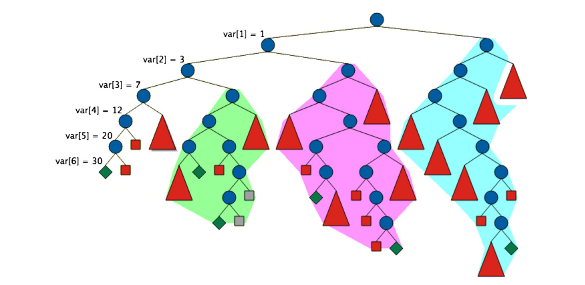
\includegraphics[width=12cm, height=6cm]{cpprofiler.png}

Cpprofiler is able to work with many different solvers by providing a standard protocol through which to interact through a tcp connection. It is then up to the maintainers of the solver to implement the protocol. This has the advantage that a visualisation of the search tree can provided before the solver has completely finished. Blue circles represent nodes with children, diamonds represent solutions, squares represent failures, triangles represent collapsed failed branches. Above each node the decision variable and the variable assignment are written. \\

Cpprofiler is difficult to navigate as it not possible to pan and zoom using the mouse. Navigating between nodes is done via arrow keys on the keyboard resulting in clumsy navigation that is frustrating to use. cpprofiler is not able to show the domains of generated variables or higher level constructs for a given node. 

\section{Methodology}

This project was originally titled conjure IDE and was open ended enough to include any possible enhancements to the conjure user's workflow. Over experimentation during the first semester I decided that I would like to focus my efforts on a search tree visualisation. Due to this period of exploration and uncertainty it would have not been possible to create a detailed plan to follow. The software engineering process that best fit this kind of project was an iterative approach. Weekly meetings with my supervisor were used to discuss progress and the direction the project was moving in. Some weeks I waas busy dealing with work from other modules and so would spend less time on the project. Other weeks I would be entirely foccussed on working on the project. However each week I would continue to make progress, even if it did not seem significant. This degree of flexibiltiy was necessary in order to manage and allocate my time efficiently. 

\section{System Design}


\subsection{Platform}
The title for this project "Conjure IDE" implies creating a new IDE from scratch. However creating a stand alone IDE is an enormous task and would require much work on aspects that are not strictly relevent to the project. 
To circumvent these issues I decided to implement the tool as an extension to the already very well established and popular Vscode text editor. This has the benefit that it is more likely for people to acutally use it since it is part of a wider ecosystem of exstensibility. The user can easily incorporate the extension into their workflow without feeling like they are a restricted to using an application that exists solely for the purpose of using conjure. For example, if the user is more comfortable using vim keybindings then they may simply install a relevent extension to vscode. Offerring a comparable number of features and flexibiltiy to a stand alone IDE would be impossible.  


\subsection{Tree Visualisation}


The aim was to create a visual representation of the search tree. Unlike cpp profiler, the tree visualisation was to be easy to use and interactive. The user is able to pan and zoom using the mouse. Clicking on a node will select that node (indicated by orange highlights). A floating panel contains the domains of the the variables in terms of either solver 




\end{document}